\documentclass[14pt,a4paper,fleqn]{extarticle}
\usepackage[T2A,T1]{fontenc}
\usepackage[utf8]{inputenc}
\usepackage[russian]{babel}
\usepackage{amsmath}
\usepackage{graphicx}
\usepackage{tabularx}
\usepackage{boldline}
\usepackage{makecell}
\usepackage{arydshln}
\usepackage{mathtools}

\graphicspath{ {./images/} }
\setlength{\mathindent}{0pt}
\setlength\parindent{0pt}


\begin{document}
	\begin{titlepage}
		
\includegraphics[scale=0.12]{logo}
		\begin{center}
			\textbf{МИНОБРНАУКИ РОССИИ}\\
			\vspace{0.2cm}
			\textbf{Федеральное государственное бюджетное образовательное учреждение высшего образования}\\
			\textbf{«САНКТ-ПЕТЕРБУРГСКИЙ ГОСУДАРСТВЕННЫЙ ЭКОНОМИЧЕСКИЙ УНИВЕРСИТЕТ»}\\
			\vspace{0.6cm}
			Факультет информатики и прикладной математики\\
			Кафедра прикладной математики и экономико-математических методов\\
			\vspace{1cm}
			\textbf{ОТЧЁТ}\\
			по дисциплине:\\
			\textbf{«Методы оптимизации»}\\
			на тему:\\
			\textbf{«Задание 19. Метод внешней точки»}\\
		\end{center}
		\vspace{1cm}
		Направление: 01.03.02\\
		Обучающийся: Бронников Егор Игоревич\\
		Группа: ПМ-1901\\
		\vfill
		\begin{center}
			Санкт-Петербург\\
			2021\\
		\end{center}
	\end{titlepage}
	\textbf{Дано:}\\
	Функция:\\
	$f = 2x_1^2 + 3x_2^2 + 4x_3^2 + 2x_1x_2 + 2x_1x_3 - x_2x_3 - 3x_1 - 5x_2 - 55x_3$\\
	
	Ограничения:\\
	$2x_1 - x_2 + x_3 = -2$\\
	$x_1 - 2x_2 + 3x_3 = -7$\\
	
	\textbf{Условие:}\\
	Найти стационарную точку методом внешней точки.\\
	
	Для начала сведём наши ограничения-равенства к неравенствам:
	\begin{center}
		$2x_1 - x_2 + x_3 < -2 + \epsilon$\\
		$2x_1 - x_2 + x_3 > -2 - \epsilon$\\
		$x_1 - 2x_2 + 3x_3 < -7 + \epsilon$\\
		$x_1 - 2x_2 + 3x_3 > -7 - \epsilon$\\
	\end{center}

	Рассмотрим следующую внешнюю штрафную функцию:
	\begin{center}
		$\Phi_4(X,C)= C\smashoperator[r]{\sum_{j=1}^{M}} (\max\{\psi_j(X), 0\})^2$
	\end{center}
	Далее составим модифицированную целевую функцию:
	\begin{center}
		$F(X, \tau) = f(X) + \tau \Phi_4(X)$
	\end{center}
	\begin{center}
		\small $F(X, \tau) = 2x_1^2 + 3x_2^2 + 4x_3^2 + 2x_1x_2 + 2x_1x_3 - x_2x_3 - 3x_1 - 5x_2 - 55x_3 +$\\
		$ + \tau ((\max \{2x_1-x_2+x_3+2-\epsilon, 0\})^2 + (\max \{-2x_1+x_2-x_3-2-\epsilon, 0\})^2$
		$ + (\max \{x_1-2x_2+3x_3+7-\epsilon, 0\})^2 + (\max \{-x_1+2x_2-3x_3-7-\epsilon, 0\})^2)$
	\end{center}
	Возьмём $X^0 = (10, 100, 10)$, которая лежит за пределами множества допустимых решений, а $\epsilon = 0.0001$.
	\newpage
	При $\tau = 10$. Для нахождения следующего приближения воспользуемся методом Ньютона-Рафсона. Таким образом, мы получили точку $X^1 = (-0.0841069, 5.32312, 1.9196)$.\\\\
	При $\tau = 100$. Воспользуемся методом Ньютона-Рафсона. Таким образом, мы получили точку $X^2 = (1.17182, 5.25464, 0.818046)$.\\\\
	При $\tau = 1000$. Воспользуемся методом Ньютона-Рафсона. Таким образом, мы получили точку $X^3 = (1.24205, 5.25048, 0.756915)$.\\\\
	При $\tau = 10000$. Воспользуемся методом Ньютона-Рафсона. Таким образом, мы получили точку $X^4 = (1.24913, 5.25005, 0.75075)$.
	\begin{center}
		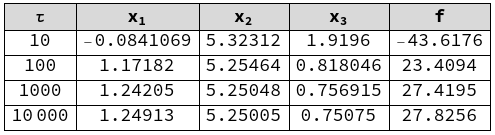
\includegraphics[scale=0.55]{pic}
	\end{center}
	
	Точный ответ: $X^* = (1.25, 5.25, 0.75), f = 27.875$
\end{document}